\documentclass{lxaiproposal}

\usepackage[english]{babel}

\PassOptionsToPackage{hyphens}{url}\usepackage{hyperref}
\usepackage{times}
\usepackage{array}
\usepackage{color}
\usepackage{epsfig}
\usepackage{pifont}
\usepackage{pifont}
\usepackage{caption}
\usepackage{float}
\usepackage{amsmath}
\usepackage{amssymb}
\usepackage{caption}
\usepackage{amssymb}
\usepackage{pdfpages}
\usepackage{makecell}
\usepackage{svg}
\usepackage{booktabs}
\usepackage{latexsym}
\usepackage{booktabs}
\usepackage{colortbl}
\usepackage{multirow}
\usepackage[compact]{titlesec}
\usepackage{tabularx}
\usepackage{subcaption}
\usepackage{xcolor}

\usepackage[T1]{fontenc}
\usepackage[latin1]{inputenc}

\setlength{\parskip}{0.1cm}
\setlength{\parindent}{0em}

\usepackage[compact]{titlesec}
\titlespacing{\section}{0pt}{2ex}{1ex}
\titlespacing{\subsection}{0pt}{1ex}{0ex}
\titlespacing{\subsubsection}{0pt}{0.5ex}{0ex}

% title config
\titleformat{\section}
  {\Large\bfseries}
  {\thesection}
  {0.5em}
  {}
\titleformat{\subsection}
  {\normalfont\large\bfseries}
  {\thesubsection}
  {0.25em}
  {}

\title{Virtual Node Graph Neural Networks for Metal-Organic Framework Inference Tasks\\}
% \large Summer 2023 PURA Salary Award Proposal}
\author{\coord{Sidharth Baskaran}{}{1}}
\address{\affil{1}{
College of Computing, Georgia Institute of Technology}}

\email{sidharth.baskaran@gatech.edu}

\begin{document}
\noindent
\maketitle

\section*{Project Overview}

In materials science, molecular property prediction has a range of applications, including
energy catalyst optimization and drug discovery. Graph neural networks (GNNs) have proven to be highly effective and scalable for such inference tasks; representing molecules as graphs and scaling to $O(n)$ runtime complexity as opposed to $O(n^3)$ for conventional methods such as density-functional theory (DFT). Metal-organic frameworks (MOFs) are porous materials consisting of metal clusters linked by organic components, and pose a challenge for GNNs as porosity is difficult to realize in graphs. We propose a model-agnostic method incorporating virtual nodes into molecular graphs MOF prediction tasks. This project is undertaken under mentorship of Dr. Victor Fung (\textit{Georgia Tech CSE}) and in collaboration with Dr. Guojing Cong (\textit{Oak Ridge National Laboratory}).

\subsection*{Message-Passing Graph Neural Networks}

Graph neural networks (GNNs) are popular in computational materials science, and can be used on a variety of tasks, including property inference, synthesis prediction, and structure generation\cite{Reiser2022}. GNNs perform convolutions over arbitrary inputs with standardized feature dimensions, and offer the advantage of working with atomic structures, which easily translate to graphs. A graph $G=(v,e,u)$ is represented by a set of nodes $v$, edges $e$, and global properties $u$. Nodes are assigned attributes ${\bf x}\in \mathbb{R}^{n}$ and edges ${\bf e}\in \mathbb{R}^m$. Message-passing (MP) GNNs propagate information between adjacent nodes $v_i,v_j$ across $e_{ij}$. Graph convolutional operators such as in CGCNN (Crystal Graph Convolutional Neural Network)\cite{Xie_2018} perform complex node attribute MP schemes of the form in (\ref{eq:mpupdate}) where for a $k$th update step, $\bigoplus$ is a differentiable, permutation-invariant reduction such as mean, max, sum, and $\gamma,\phi$ are multilayer perceptrons (MLPs)\cite{sanchez-lengeling2021a}.
\begin{equation}
    \textstyle
    \mathbf{x}_i^{(k)} = \gamma^{(k)} \left( \mathbf{x}_i^{(k-1)}, \bigoplus_{j \in \mathcal{N}(i)} \, \phi^{(k)}\left(\mathbf{x}_i^{(k-1)}, \mathbf{x}_j^{(k-1)},\mathbf{e}_{j,i}\right) \right)
    \label{eq:mpupdate}
\end{equation}

Each atom is a node in the graph, and is assigned a vector of node attributes encoding chemical properties. Bonds are represented by edges and are assigned vector attributes encoding spatial info (\ref{fig:unitcellmp}). Molecular property inference involves scalar-valued predictions given graph inputs. Our pipeline consists of convolutional layers followed by fully-connected layers to provide a global readout value (\ref{fig:pipeline}).

\begin{figure*}
    \centering
    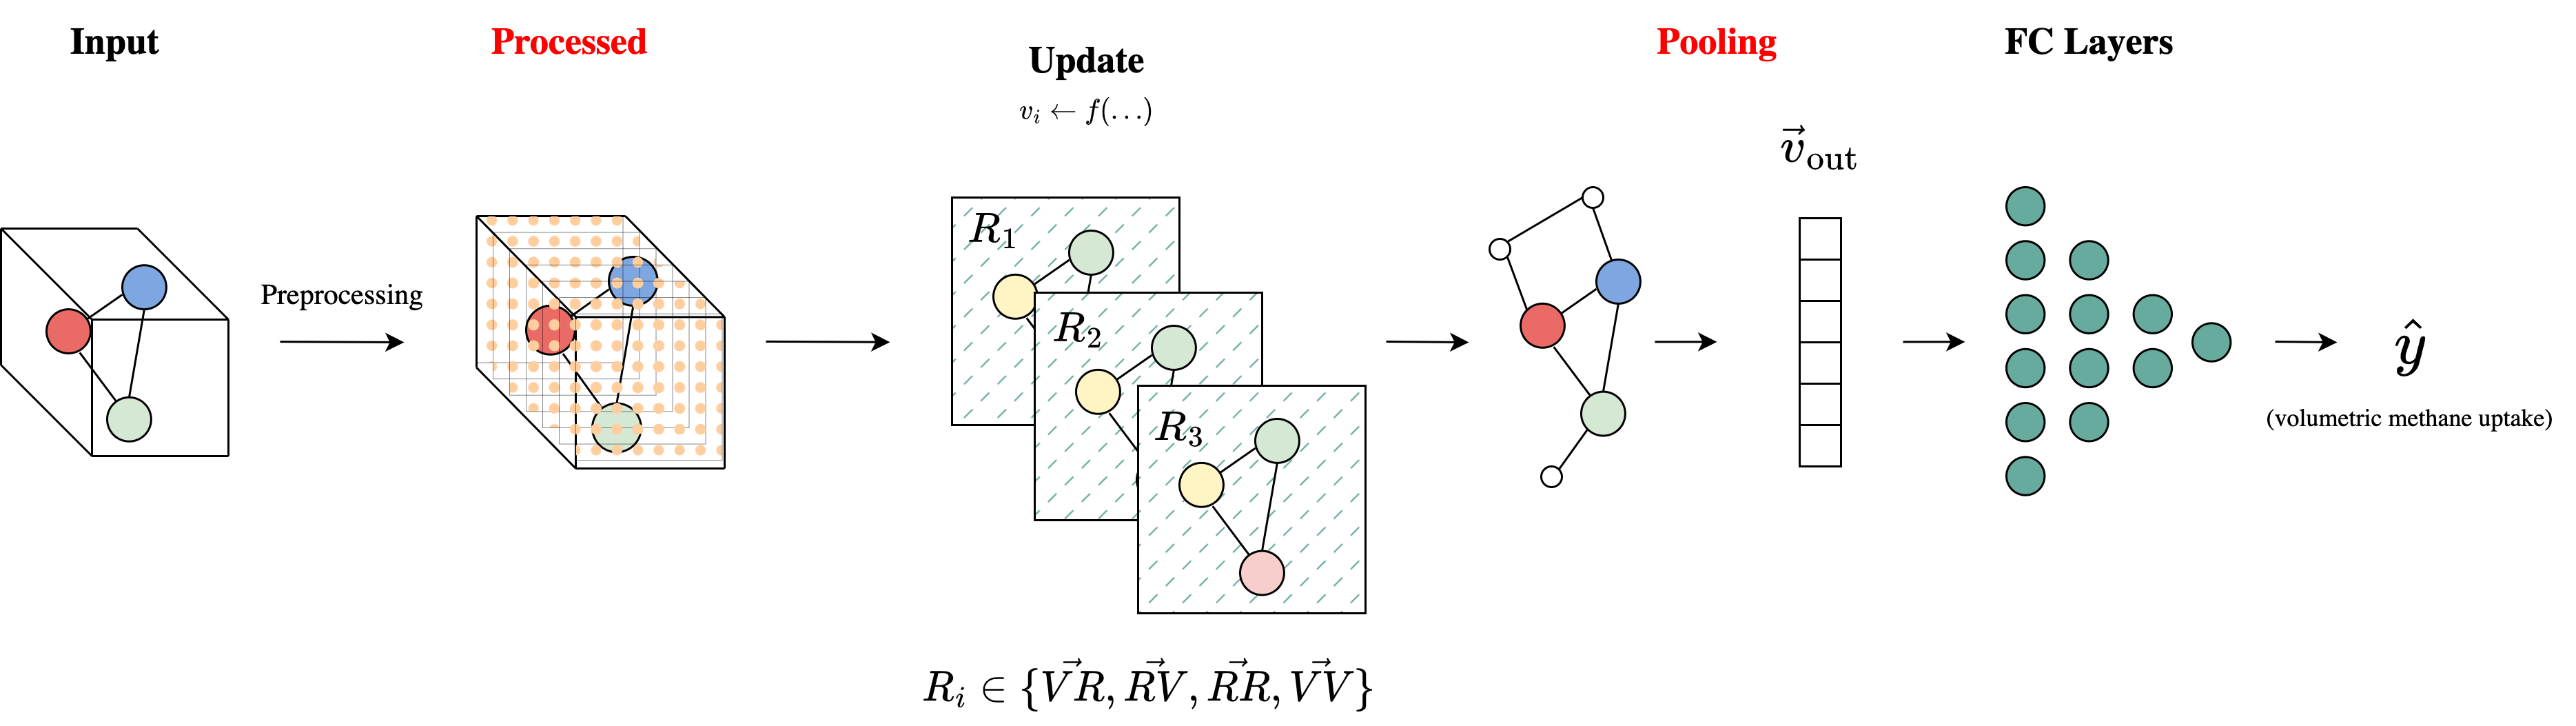
\includegraphics[width=0.8\textwidth]{mdl-vn-pipeline.drawio.png}
    \caption{Volumetric methane uptake inference pipeline with virtual nodes in MatDeepLearn\cite{fung2021benchmarking}}
    \label{fig:pipeline}
\end{figure*}

\subsection*{hMOF Dataset}

Metal-organic frameworks (MOFs) are composed of modular building blocks, known for porosity and stability. The space of  MOFs is large due to modular combinations. The hypothetical metal-organic framework (hMOF) generation procedure generates every possible structure under constraints to produce 137,953 hMOFs, using building blocks of naturally occurring MOFs. The global properties for each structure are surface area, pore volume, pore-size distribution, powder X-ray diffraction pattern, and methane-adsorption capability\cite{wilmer2012large}.

\subsection*{Virtual Nodes for Graph Structures}

Crystal structures are an infinite system GNNs use the graph of the smallest repeating unit (unit cell) as an approximation for the system, described by a set of basis vectors. Virtual nodes are throughout the unit cell parallelepiped to form a controllable mesh (\ref{fig:unitcellmp}). Each virtual node is described by a node attribute vector and is connected via edges to real and virtual nodes (\ref{fig:unitcellmp}). This approach introduces a set of hyper-parameters (\ref{table:vn-hparam}) in addition to those of the candidate model (i.e. CGCNN).

\section*{Research Plan and Methods}

\subsection*{Preliminary Results}

Without virtual nodes, we use $R=\{\vec{RR}\}$ with an interaction of 5 A$^\circ$.
Baseline tests for virtual nodes were done with $R=\{\vec{RV},\vec{RR}\}$ with interaction cutoff of 5 A$^\circ$, virtual box increment of 3 A$^\circ$, atomic-number based pooling, and umean reduction. The candidate model used was CGCNN. 5000 examples from the hMOF dataset were used, with training, testing, and validation splits of 0.85, 0.15, and 0.05 respectively. Results are shown in Figure (\ref{plot:prelim-results}), indicating that virtual nodes provide a significant improvement on prediction of volumetric methane uptake.

\subsection*{Hyper-parameter Optimization}

In order to further improve performance from the baseline, our approach will involve virtual node-specific (\ref{table:vn-hparam}) hyper-parameter tuning to identify the most influential parameters.
Specifically, the readout and pooling phase of the model also high potential for improvement through combining different pooling schemes with methods that take advantage of virtual nodes, potentially including attention-based and hierarchical approaches\cite{zhang2019hierarchical}. A current limitation with our readout phase is the high dimensional reduction occurring from the atomic number pooling scheme, which involves a mapping from a $kn$ size feature vector $\vec v_\text{out}$ to a set of fully-connected layers mapping $\approx n\to 1$ (\ref{fig:pipeline}). We are currently working on methods to address this loss of expressiveness, where $k$ can be as much as $100$. Furthermore, current developments in the GNN space offer model architectures with significant efficiency and performance improvement over CGCNN, providing better options for virtual-node candidates, such as equivariant networks that encode angular information\cite{jorgensen2022equivariant}.

\subsection*{Heterogeneous Graphs}

Heterogeneous graphs provide a way to separate different classes of nodes and edges and learn a separate set of model weights for each class and allow for different types of interactions in one end-to-end task. Treating virtual nodes and real nodes as separate classes allows each class to incorporate a separate set of model weights, improving expressiveness and allowing each class to incorporate a different method of encoding node and edge features. While this increases complexity and memory overhead, approaches such as parallelization over multiple GPUs and transfer learning are possible solutions. Further possibilities include combining or chaining different GNN models across heterogeneous classes to improve expressiveness.

\subsection*{Methods}

Pre-processing and training utilizes MatDeepLearn\cite{fung2021benchmarking}, software I actively help develop in collaboration with the Fung Group. We a single NVIDIA A100 40GB or A40 48GB GPUs to train models on HPC clusters provided by National Energy Research Scientific Computing Center's Perlmutter supercomputer, and PACE Hive and Phoenix clusters\cite{PACE}. We utilized PyTorch\cite{pytorch} and PyTorch Geometric for graph learning and optimized sparse tensor arithmetic \cite{Fey2019FastGR}, and Weights and Biases\cite{wandb} automated hyper-parameter tuning and experiment tracking.

\section*{Related Work}

Machine learning-based approaches to predict methane-adsorption exist, but do not utilize GNNs, rather creating structural fingerprint vectors encoding spatial and chemical information. Deep neural networks are then used to map these fingerprints to predicted methane-adsorption. \cite{gurnani2021interpretable}. 
Virtual nodes have been used in GNNs for materials property inference, but for different use cases including full phonon\cite{https://doi.org/10.48550/arxiv.2010.09435} and electron density prediction\cite{jorgensen2022equivariant}.

\begin{figure}[h]
    \centering
    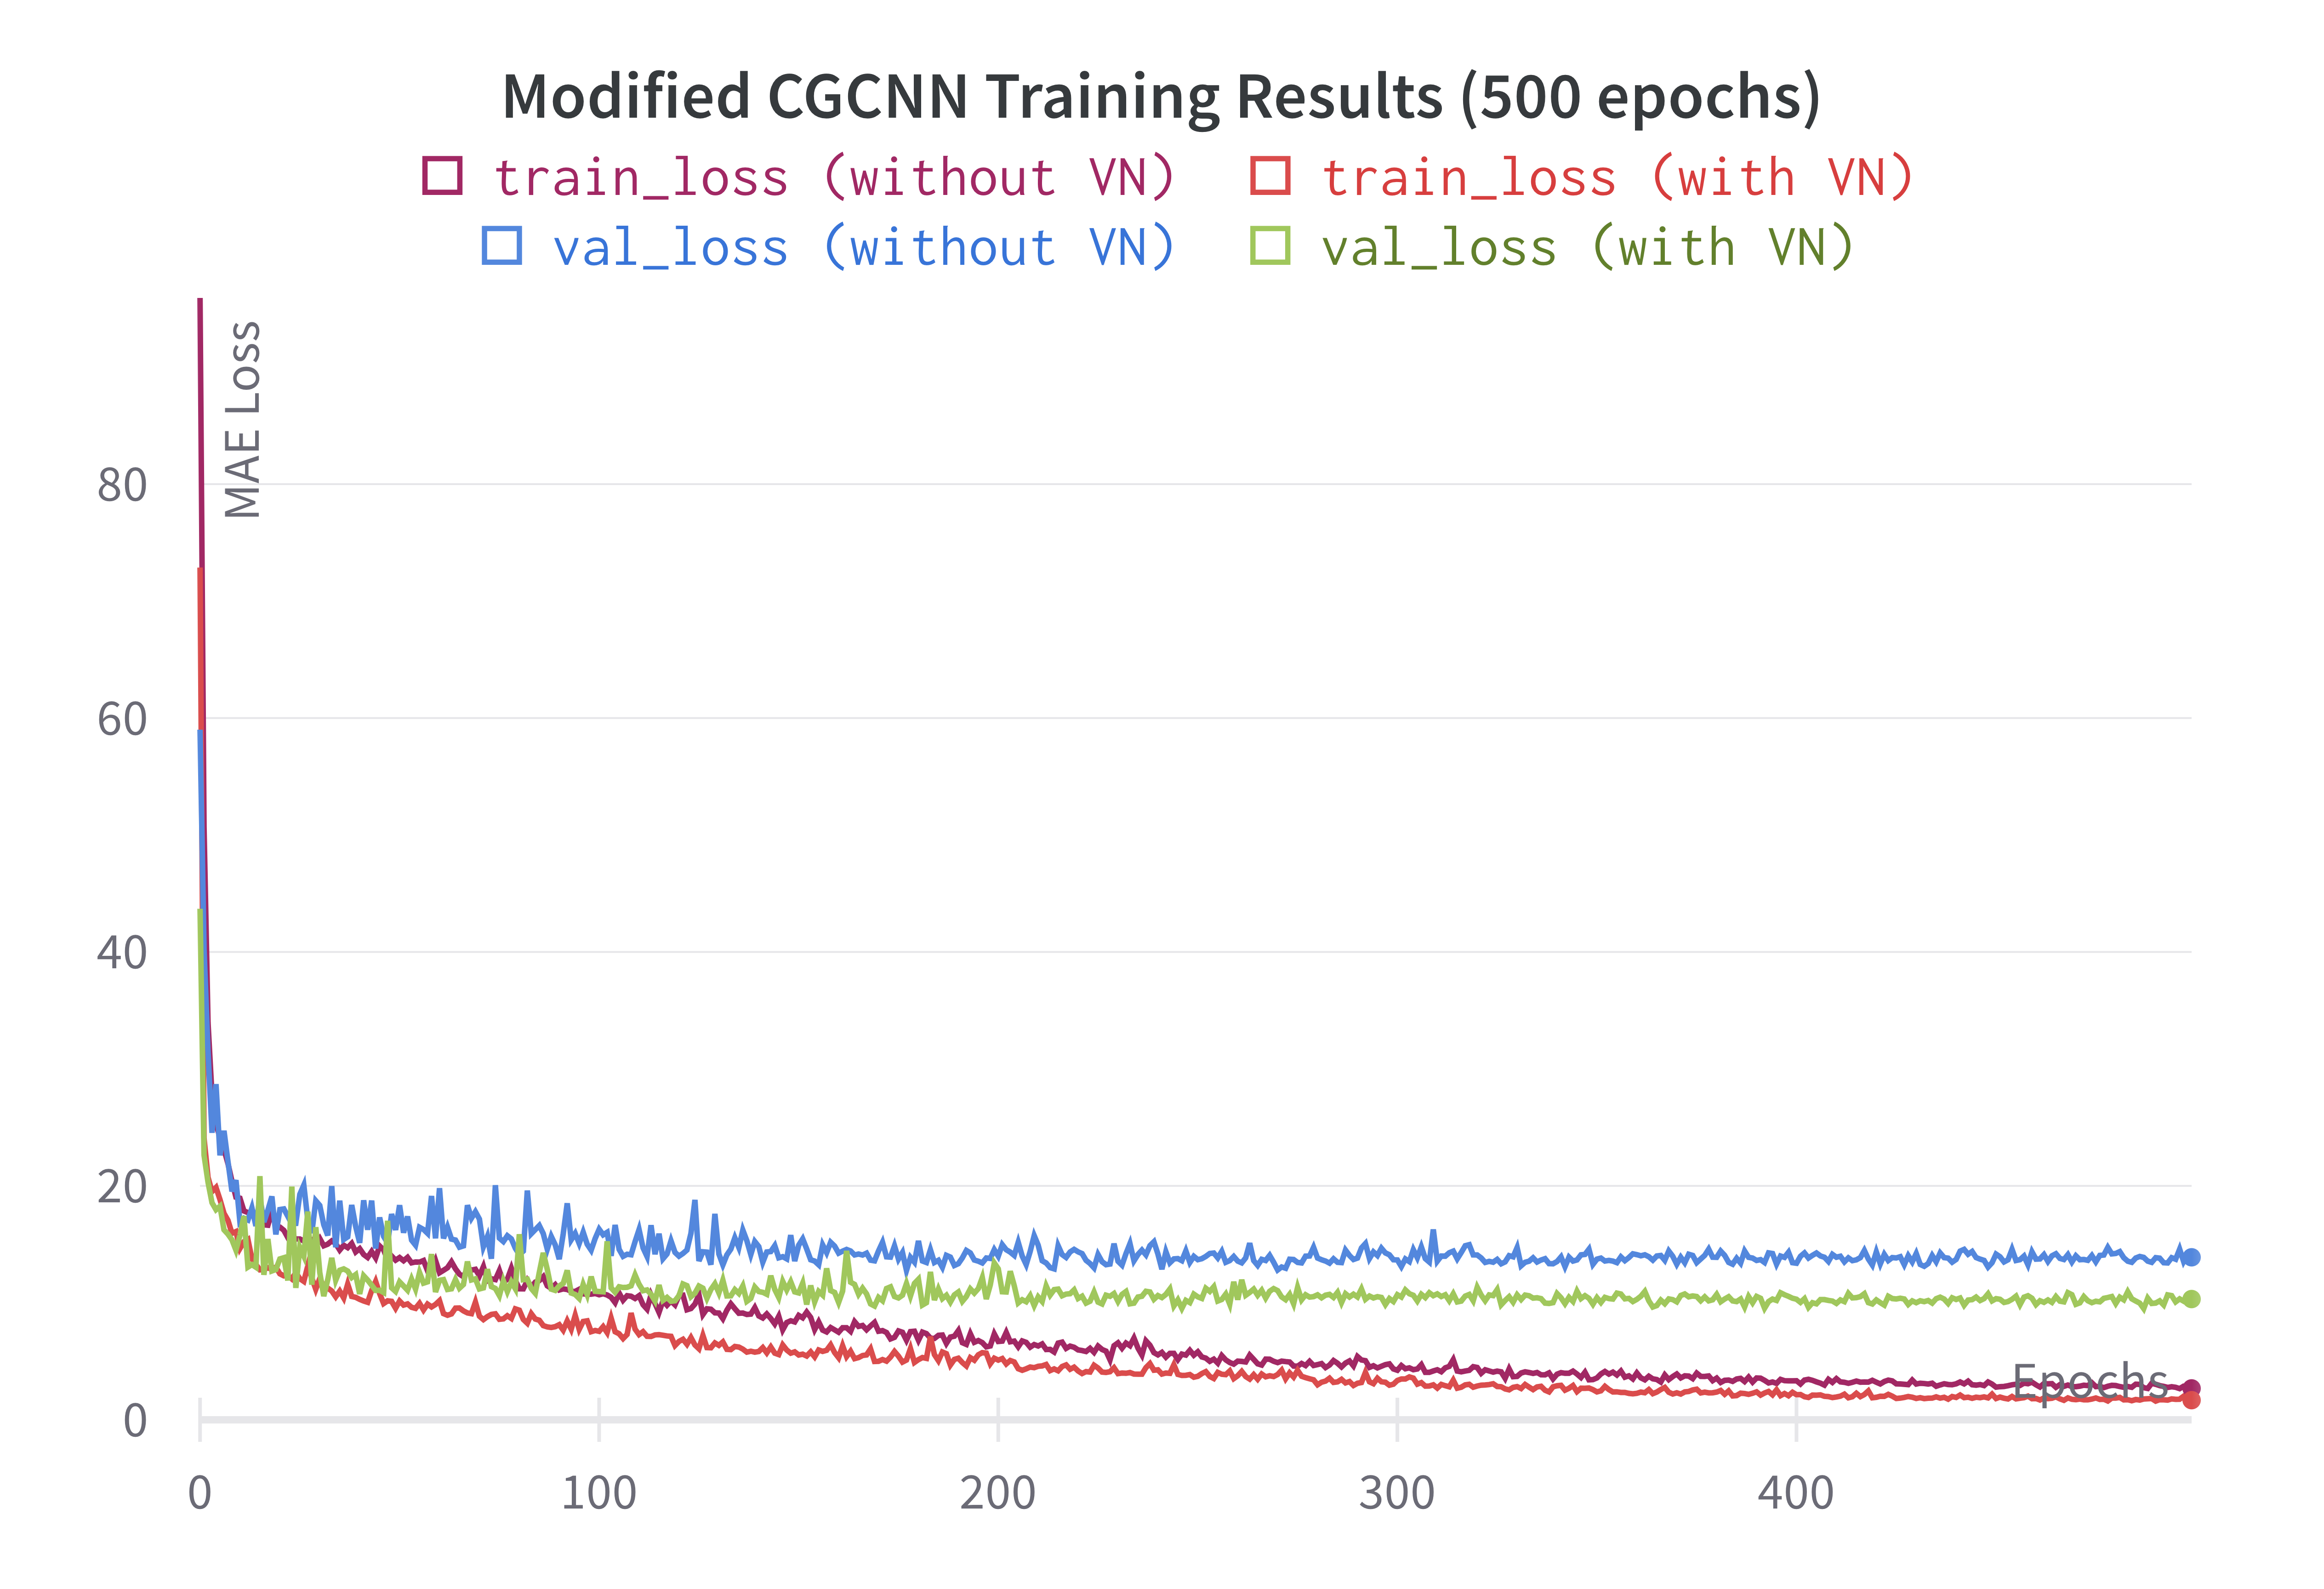
\includegraphics[width=0.9\linewidth]{result-plots-wandb.png}
    \caption{Training results on CGCNN model (lower is better)}
    \label{plot:prelim-results}
\end{figure}

\begin{table}[h]
        {\scriptsize\begin{tabularx}{\linewidth}{p{0.2\linewidth} p{0.05\linewidth} p{0.6\linewidth}}
            \toprule
            \multicolumn{1}{c}{\textbf{Parameter}} & \multicolumn{1}{c}{\textbf{Unit}} & \multicolumn{1}{c}{\textbf{Description}} \\
            \midrule
            Virtual box increment & A$^\circ$ & Spacing between virtual nodes along each dimension of unit cell \\
            MP selectivity & -- & Interaction possibilities at each convolution layer, formally $R\subset I = \{\vec{RV},\vec{RR},\vec{VR},\vec{VV}\}$\\
            Interaction cutoff radius & A$^\circ$ & Cutoff radius for message-passing for each $m\in I$.\\
            Pooling method & -- &  1) Separate pooling on virtual and real nodes, followed by concatenating the results. 2) Given each atomic number, create a separate embedding size $n$ to create a $kn$ size vector for $k$ different atomic numbers.\\
            Pooling scheme & -- & Permutation invariant like sum, mean, min, max.\\
            \bottomrule
        \end{tabularx}}
        \caption{Virtual-node-specific hyper-parameters}
        \label{table:vn-hparam}
\end{table}

\begin{figure}[H]
    \centering
    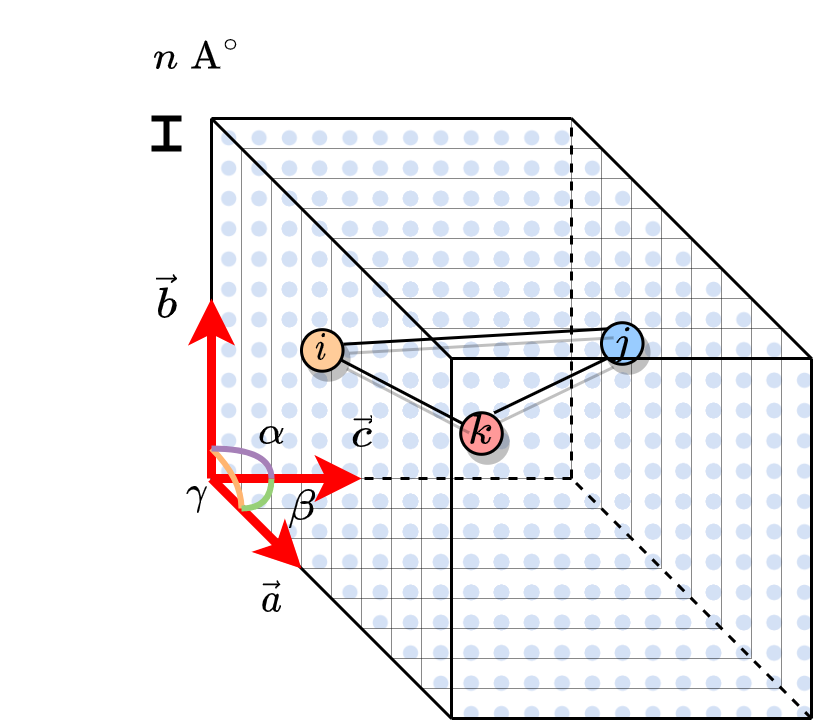
\includegraphics[width=\linewidth]{unitcell-vn.drawio.png}
    \caption{(a) Unit cell with virtual node mesh of $n$ A$^\circ$ spacing and (b) message passing scheme}
    \label{fig:unitcellmp}
\end{figure}

\newpage

\bibliographystyle{ieee_fullname}
\bibliography{references}

\end{document}